\documentclass[11pt]{article}
\usepackage{tikz}
\usepackage{pgffor}
\usetikzlibrary{shapes}
\usetikzlibrary{arrows}
\usetikzlibrary{trees}
\usetikzlibrary{patterns}

\begin{document}

\begin{figure}
\begin{center}

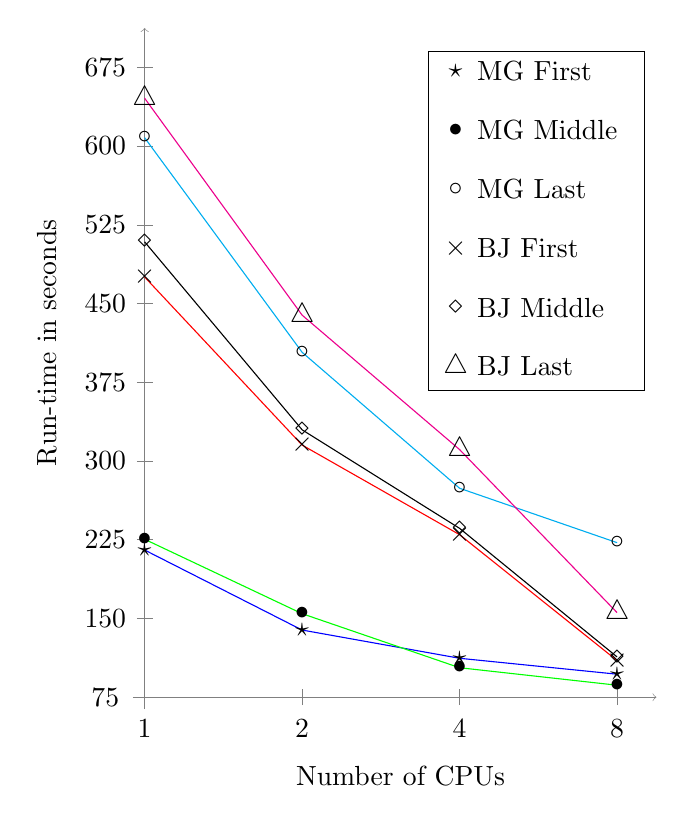
\begin{tikzpicture}[scale=1.0]

\draw[very thin, color=gray, ->] (-0.15, 0) -- (6.5, 0);
\draw[very thin, color=gray, ->] (0, -0.15) -- (0, 8.5);

\draw (3.25, -1) node {{Number of CPUs}};
\draw[color=white] (-1, 4) -- +(90:1) node[midway,sloped,above, color=black]{{Run-time in seconds}};

%Draw Row Ticks
\foreach \pos/\val in {0/1, 2/2, 4/4, 6/8} {
\draw[very thin, color=gray] (\pos, -0.1) -- (\pos, 0.1);
\draw (\pos, -0.4) node {{\val}};
}

%Draw Col Ticks
\foreach \pos/\val in {0/75, 1/150, 2/225, 3/300, 4/375, 5/450, 6/525, 7/600, 8/675} {
\draw[very thin, color=gray] (-0.1, \pos) -- (0.1, \pos);
\draw (-0.5, \pos) node {{\val}};
}

%Draw legend
\path (0.35,-0.5) coordinate (off);

\draw (off) ++ (3.25, 4.4) rectangle ++ (2.75, 4.3);
\draw (off) ++ (3.75, 4.7) node[right] {BJ Last};
\draw (off) ++ (3.75, 5.45) node[right] {BJ Middle};
\draw (off) ++ (3.75, 6.2) node[right] {BJ First};
\draw (off) ++ (3.75, 6.95) node[right] {MG Last};
\draw (off) ++ (3.75, 7.7) node[right] {MG Middle};
\draw (off) ++ (3.75, 8.45) node[right] {MG First};

\draw (off) ++ (3.6, 4.7) node {$\triangle$};
\draw (off) ++ (3.6, 5.45) node {$\diamond$};
\draw (off) ++ (3.6, 6.2) node {$\times$};
\draw (off) ++ (3.6, 6.95) node {$\circ$};
\draw (off) ++ (3.6, 7.7) node {$\bullet$};
\draw (off) ++ (3.6, 8.45) node {$\star$};



\draw[blue]
 (0.000000, 1.869687) --
 (2.000000, 0.853445) --
 (4.000000, 0.494788) --
 (6.000000, 0.292686) ;

 \draw (0.000000, 1.869687) node {$\star$};
 \draw (2.000000, 0.853445) node {$\star$};
 \draw (4.000000, 0.494788) node {$\star$};
 \draw (6.000000, 0.292686) node {$\star$};


\draw[green]
 (0.000000, 2.006217) --
 (2.000000, 1.061307) --
 (4.000000, 0.374791) --
 (6.000000, 0.152810) ;

 \draw (0.000000, 2.006217) node {$\bullet$};
 \draw (2.000000, 1.061307) node {$\bullet$};
 \draw (4.000000, 0.374791) node {$\bullet$};
 \draw (6.000000, 0.152810) node {$\bullet$};


\draw[cyan]
 (0.000000, 7.105956) --
 (2.000000, 4.380957) --
 (4.000000, 2.654067) --
 (6.000000, 1.962884) ;


 \draw (0.000000, 7.105956) node {$\circ$};
 \draw (2.000000, 4.380957) node {$\circ$};
 \draw (4.000000, 2.654067) node {$\circ$};
 \draw (6.000000, 1.962884) node {$\circ$};



\draw[red]  (0.000000, 5.336933) --
 (2.000000, 3.202587) --
 (4.000000, 2.064482) --
 (6.000000, 0.465455) ;

\draw (0.000000, 5.336933) node {$\times$};
\draw (2.000000, 3.202587) node {$\times$};
\draw (4.000000, 2.064482) node {$\times$};
\draw (6.000000, 0.465455) node {$\times$};


\draw[black] (0.000000, 5.783589) --
 (2.000000, 3.396582) --
 (4.000000, 2.144880) --
 (6.000000, 0.511854) ;

\draw (0.000000, 5.783589) node {$\diamond$};
\draw (2.000000, 3.396582)  node {$\diamond$};
\draw (4.000000, 2.144880)  node {$\diamond$};
\draw (6.000000, 0.511854)  node {$\diamond$};


\draw[magenta]
 (0.000000, 7.607276) --
 (2.000000, 4.852679) --
 (4.000000, 3.145121) --
 (6.000000, 1.074640) ;


\draw  (0.000000, 7.607276) node {$\triangle$};
\draw  (2.000000, 4.852679) node {$\triangle$};
\draw  (4.000000, 3.145121) node {$\triangle$};
\draw  (6.000000, 1.074640) node {$\triangle$};


\end{tikzpicture} 

\end{center}
\end{figure}

\end{document}
			